\section{The Interstellar Medium}

I added sections based on the list of important topics Allison gave us 
before the final. 

\subsection{Questions}
\begin{enumerate}
\item \textbf{Draw the cooling function for gas of solar metallicity, and describe the cooling
      mechanisms in each part of the curve. Explain the relevance of this function to multi-
      phase ISM models.}
      
      Figure \ref{f:cool1} shows the cooling function $\Lambda$ as a function of $T$ (note that in class, Nick showed us a cooling curve of $T$ vs. $n$). At $T < 10^3$ K, the cooling is from molecular line emission. The plateau from $\sim10^3$ to $\sim10^4$ K is due to collisionally excited lines of neutral and low-ionization metals. There is a peak around $\sim10^4-10^5$ K, which is due to recombination of hydrogen (i.e. hydrogen recombines and then downward transitions emit low-energy photons such as H$\alpha$ that find the HII region optically thin). There is a quadruple peak at $T \approx 10^5,~2\times 10^5,~5\times 10^5,~10^6$ K from far-UV and X-ray emission lines from highly ionized species of C,O,Ne,Fe, respectively. At $T > 10^7$ K, most of the cooling is from Bremsstrahlung.
      
      \begin{figure}[ht]
      \begin{center}
      \includegraphics[width=\textwidth]{ism_Q1_cool.jpg}
      \end{center}
      \caption{Cooling curve from Astrophysics in a Nutshell. \label{f:cool1}}
	  \end{figure}
	
	  Figure \ref{f:cool2} is a more detailed version from Nick's notes, and it goes to higher temperature.
	
	  \begin{figure}[ht]
      \begin{center}
      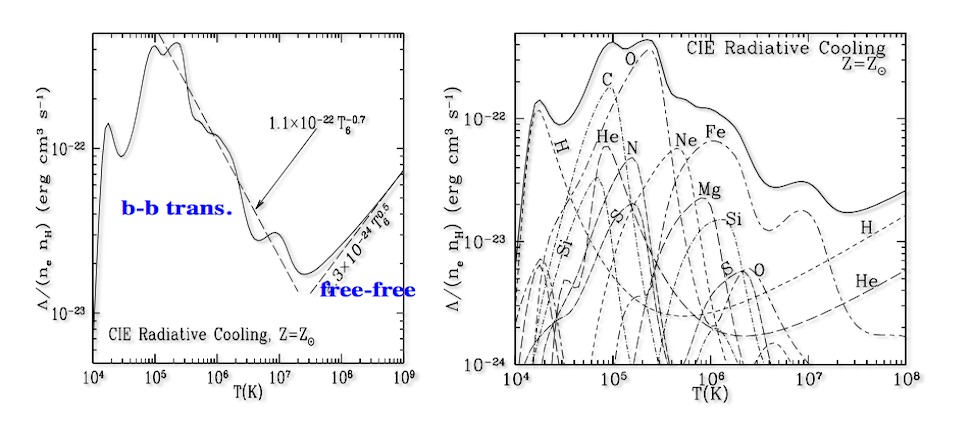
\includegraphics[width=\textwidth]{ism_Q1_cool_b.jpg}
      \end{center}
      \caption{Cooling curve from Nick's notes with more details on relevant elements. \label{f:cool2}}
      \end{figure}

      \newthought{So how does} the cooling function relate to the multi-phase\sidenote{
            Here we take ``phase'' to mean a particular temperature, density, and ionization
            state of the ISM.  I (Michael) believe we use the word ``phase'' to indicate that not
            all combinations of temperature and density are possible -- there are distinct
            regions of phase-space that define the characteristics of the ISM.
      } nature of the ISM?
      To understand this, let's suppose the ISM is composed of two or more distinct phases.
      The boundary between these two phases (assuming the boundary between them is at least
      quasi-stable) must satisfy pressure equilibrium such that $n_1T_1=n_2T_2$.  Additionally,
      each phase must have cooling balanced by heating, and be stable to temperature
      perturbations\sidenote{
            This means that if the temperature is increased, cooling dominates heating, and if
            the temperature is decreased, heating dominates cooling.
      }.
      Therefore, areas where the cooling function decreases as a function of temperature
      (cooling increases as temperature decreases) are likely to be unstable.  However, for a more
      detailed treatment of cooling and heating, one must consider the balance $n^2\Lambda(T) = n\Gamma(T)$
      for an arbitrary cooling function $\Lambda$ and heating function $\Gamma$.
      
\item \textbf{Draw a typical spectrum of an HII region, including both lines and continuum, and
      explain the major processes that give rise to each feature.}
      
      Figure \ref{f:HIIspec} shows a spectrum of an HII region with the continuum removed. The spectrum is similar to that of a planetary nebula (a ball of mostly-hydrogen gas ionized by the newly formed white dwarf instead of a young star). The hydrogen features are from transitions to the $n=2$ state (no Lyman features are pictured here, but ${\rm Ly}\alpha$ should be there) of 
      
      \begin{figure}[ht]
      \begin{center}
      \includegraphics[width=\textwidth]{ism_Q2_HII_spec.jpg}
      \end{center}
      \caption{Spectrum of an HII region with the continuum removed. \label{f:HIIspec}}
	\end{figure}
	
	 The spectrum is similar to that of a planetary nebula (a ball of mostly-hydrogen gas ionized by the newly formed white dwarf instead of a young star). The Hydrogen features are from transitions to the $n=2$ state (no Lyman features are pictured here, but ${\rm Ly}\alpha$ should be there). 
	 
	 The other prominent features are from singly- and doubly-ionized Oxygen bound-bound transitions. These ions are important coolants in HII regions and act as thermostats for the gas. Free electrons zooming around will collisionally excite the Oxygen ions to an excited state, which will then decay and radiate line emission. The gas is optically thin to these lines, so they are very prominent in the spectra. 
	 
	 \emph{An Explanation of Oxygen Cooling in HII Regions--} The Oxygen ions help maintain the temperature of the HII region at a steady 10,000 K. This is because they are collisionally excited. If the gas is hotter than 10,000 K, the increased velocity of the free electrons increases the number of collisions, converting the excess kinetic energy into line emission which escapes the gas. If the gas is cooler than 10,000 K, the lower velocity reduces the number of collisions, and hence the amount of cooling. This allows the gas opportunity to gain energy and increase its temperature back up to 10,000 K.\emph{end side note}
	 
	 The continuum from the HII region is from the star, and from recombination. I wish I had figures of either of these but I couldn't find any. The star's blackbody is modified as the Hydrogen absorbs any wavelength shortward of the Lyman limit of 912\AA. Remember that wavelengths closer to that number are absorbed preferentially, so photons of much higher energy are not attenuated as much. This manifests as a sharp drop of stellar flux at the Lyman limit, and then a slight rise toward shorter wavelengths. I actually found a figure of this situation but I forgot which book it was in and couldn't find it again... Basically this is what makes the stellar spectrum 'harder' toward the edge of the HII region: all the flux right at the Lyman limit has been absorbed, so the far UV flux is higher than the near UV flux. The longer wavelengths of the star's spectrum is mostly left untouched.
	 
	 As Hydrogen can be ionized by many possible wavelengths, the free electrons that result can have a continuum of energies. This also means that when one of these free electrons recombines with Hydrogen, the first photon it releases can have a continuum of energies. This is called the "recombination continuum". Unfortunately I have no idea what it looks like in a spectrum...
	 
	 
\item \textbf{Explain quantitatively what determines the temperature of dust grains and their
      thermal emission spectrum. Give examples of astrophysical environments with different
      dust temperatures.}
\end{enumerate}

	First, let's remember what dust is. Dust grains are macroscopic particles of mostly ices and metals in solid form. With radii of $r \sim 1 nm - 0.1 \mu m$, they are around the same size of what we'd consider 'smoke'. Because they are macroscopic, their emission is based on their \textbf{temperature}. A gas's temperature is determined by interactions with a radiation field, but also by collisions between the particles. Dust temperature, however, is only determined by equilibrium with the radiation field. Hence, \emph{mixed gas and dust can have different temperatures}. 
	
	Dust absorbs preferentially bluer light, depending on the grain's size. In class we had a homework problem where the fraction of light absorbed was defined as:
	
	\begin{equation}
	Q_{abs} = (\frac{2\pi a}{\lambda})^{n}
	\end{equation}
	
	where $a$ is the radius of the dust grain, and $n$ is a positive number. If the grain is very large, or the photon wavelength is very small, all light will be absorbed. This quantity comes into play in the definition of the dust absorption coefficient:
	
	\begin{equation}
	\kappa_{\lambda} = \pi a^{2} Q_{abs} n_{dust}
	\end{equation}
	
	For the typical sizes of dust grains, in a region where the incident flux is dominated by UV light, one can approximate as all the incident flux being absorbed by the dust. 
	
	This coefficient, in a detailed treatment, also affects the emission of the dust grain, where:
	
	\begin{equation}
	j_{\lambda} = \kappa_{\lambda} B_{lambda}(T_{dust})
	\end{equation}
	
	This describes the emission as a blackbody at equilibrium dust temperature $T_{dust}$ modified by the opacity. 
	
	In the approximation that the dust emits completely like a blackbody, $n = 1$ and one finds the temperature of the dust as function of distance from a nearby star:
	
	\begin{equation}
	T_{dust}(r) = \sqrt{\frac{R_{*}}{2r}}T_{*}
	\end{equation}	
	
	

\subsection{Useful Numbers and Relations}
$2\times10^{21}$ H cm$^{-2}$ for $1$ mag of visual extinction\newline
\newline
$30$ mag of visible extinction towards Galactic Center\newline
\newline
$13.6$ eV=$912$ \AA=shock with v$>50$ km/s\newline
\newline
$\frac{E}{eV}=\frac{T}{10,000 K}$\newline
\newline
H photoionization cross section $\sigma_{\nu}=6\times10^{-18}(\nu/\nu_0)^{-3}
cm^2$\newline
\newline
mean free path = $1/(n\sigma)\sim 1.6\times10^{17}/n_H$ cm\newline
\newline
$v_{sound}=\sqrt{\frac{\gamma kT}{m}}$\newline
\newline
For atomic H and $\gamma=5/3$,\newline
\newline
$\frac{v_{sound}}{km/s}=\sqrt{\frac{T}{100 K}}$

\subsection{Basic Things about ISM Phases}

The ISM phases are characterized by the state of hydrogen gas.

H$_2$ (molecular): $n \sim 200-10^6~{\rm cm}^{-3}$, $T \sim 10-500~{\rm K}$

Exists in molecular clouds and dark clouds, as well as protostellar cores.  
Molecular and dark clouds (lower end of the temperature and density range) are 
detected based extinction of background stars.  Giant molecular clouds 
have temperatures of $50-100$ K and and are heated by newly formed massive 
stars.  These are also seen in extinction, and in line emission in the far-IR 
and radio.  The molecular H itself is very difficult to detect 
spectroscopically, but other molecules in the clouds such as CO can be 
detected.  Giant molecular clouds have masses of 
$10^3-10^6\ M_{\odot}$.  The hottest and densist H$_2$ is found in protostellar 
cores, which are collapsed regions of GMCs.  

HI (atomic): $n \sim 1-100~{\rm cm}^{-3}$, $T \sim 100-3000~{\rm K}$

Atomic H is found in diffuse clouds.  These clouds are semitransparent, with 
visual extinction of $\sim1$ mag.  The are observed using $21$ cm emission 
(warmer clouds) and absorption (cooler clouds).  In the centers of the clouds, 
molecules such as CO and OH can form and be shielded from starlight.  These 
clouds are also visible in the infrared from their blackbody radiation.  
 
HII (ionized): $n \sim 0.1-10^3~{\rm cm}^{-3}$, $T \sim 10^4-10^6~{\rm K}$

Ionized H is found in emission nebulae (planetary nebulae, supernova remnants, 
and HII regions).  Observationally, ionized H can be observed using H 
recombination lines (such as H$\alpha$) and other atomic recombination lines 
such as [OIII].  Bremsstrahlung emission is also seen in these regions.  
Supernova remnants and planetary nebulae have well defined shell-like shapes 
and are associated with individual stars.  HII regions appear fuzzy and 
are associated with sites of multiple star formation and molecular clouds.  
Planetary nebulae can also be distinguished from HII regions from line ratios.  
The star at the center of a planetary nebula is the core of an evolved star, 
and can be $>10^5$ K.  This produces much higher energy photons than those 
in HII regions, so ratios of [OIII] to H$\alpha$ are higher in planetary 
nebulae, and even He recombination lines are weakly visible.  

Ionized H can also be found in galactic coronal gas in the halo.  This gas 
is most likely heated $10^5-10^6$ K gas is most likely heated by shocks from 
multiple supernovae.  It can be detected from X-ray emission and UV absorption.
 
 Transitions between phases:
 
 Ionization of neutral hydrogen requires $13.6~{\rm eV}$, or photons with wavelength $\lambda < 912 \AA$, OR shocks that are faster than $50~{\rm km/s}$. In HII regions around hot (O,B) stars, the hydrogen is photoionized by the UV radiation from the star, and there are very sharp transitions between the HII, HI, and H$_2$ regions around the star.

\subsection{Heating and Cooling}
The example of heating and cooling we did in class was for an HII region.  
According to the slides, the same derivation can be followed for other 
phases of the ISM, just with different transitions.  

In an HII region, gas is heated when a photon with energy $>13.6$ eV ionizes 
a neutral H atom.  This gives the free electron extra kinetic energy, which 
it transfers to the gas.  The rate of heating is just the rate at which 
energy is transferred into the gas by this method.  So the heating rate 
$\Gamma$ is the photo-ionization rate times the extra energy per 
photo-ionization.
\begin{equation}
\Gamma=R_{ph}\times\bar{E}
\end{equation}
Since the HII region is fully ionized, photo-ionizations can only take 
place at the rate of recombinations (this is basically saying ionization 
equilibrium is maintained.  So the rate of photo-ionizations equals the rate 
of recombinations:
\begin{equation}
R_{ph}=n_en_p\alpha_B
\end{equation}
where $\alpha_B$ is the recombination rate coefficient into levels higher than 
n$=1$.  Things get confusing here with these $\alpha$s.  There's a total $\alpha$ 
for all recombinations, an $\alpha_A$ for recombinations to n$=1$, and 
$\alpha_B$.  Kwok says $\alpha_B$ should be used here.  The lecture slides 
say it should be $\alpha_A$, but later in the derivation, it looks like this 
magically turns into $\alpha_B$.  I'm assuming the $\alpha_A$ in the lecture 
slides is a typo, and we should be using $\alpha_B$.  This makes sense 
physically, because we want to know the rate of recombinations that allow 
a photon from the central star to ionize an atom.  If a recombination happens 
directly to n$=1$, then a photon will be emitted with enough energy to 
ionize a new atom.  So the photon from the star that is trying to heat the gas 
will still have nothing new to ionize.  If the recombination happens to a 
higher energy level, and the electron cascades down to n$=1$, several photons 
will be emitted, but none will be able to ionize anything.  So the net result 
is there is now a new neutral atom that can be ionized by the star.  If this 
is all still too confusing, we can probably get away with just saying $\alpha$ 
and ignoring this whole A or B business. 

Meanwhile, back at the ranch, we need the average energy given to an electron 
in a photo-ionization.  The kinetic energy given to the electron by a photon 
of frequency $\nu$ is just $h(\nu-\nu_0)$ where $\nu_0$ is the frequency 
required to ionize H.  The total energy added by this frequency is the 
energy from one photon times the number of photons at that frequency, given 
by the intensity of the radiation field divided by the photon energy.  
Integrating over all frequencies above the ionization frequency, and dividing 
by the total number of photons gives the average kinetic energy given.   
\begin{equation}
\bar{E}=\frac{\int_{\nu_0}^\infty{h(\nu-\nu_0)\frac{J_{\nu}}{h\nu}a_{\nu}\,d\nu}}{\int_{\nu_0}^\infty{\frac{J_{\nu}}{h\nu}a_{\nu}\,d\nu}}
\end{equation}
$a_{\nu}$ is the photo-ionization cross section.  Defining $T_i$ such that 
\begin{equation}
\bar{E}=\frac{3}{2}kT_i
\end{equation}
results in 
\begin{equation}
\Gamma=n_en_p\alpha_B\frac{3}{2}kT_i
\end{equation}
For $J_{\nu}$ from a central star of temperature $T_*$ and 
$a_{\nu}\propto\left(\frac{\nu}{\nu_0}\right)^3$, $T_i\sim T_*$.

One way an HII region can cool is through recombination to energy levels 
above n$=1$, followed by a cascade to n$=1$.  Assuming all the H in the region 
is in the ground state, the emitted photons will escape the HII region, and 
kinetic energy will have been removed.  The rate at which this happens is 
\begin{equation}
\Lambda=n_en_pkT\beta
\end{equation}
where 
\begin{equation}
\beta=\alpha_B\int_0^\infty{\frac{1}{2}mv^2\frac{\sigma_vv}{kT_e}f(v)\,dv}
\end{equation}
The integral includes the kinetic energy lost by the electron, $\sigma v$, 
which has appeared in rate equations before that we've had (I don't remember 
why), and the distribution of velocities.  Re-writing the cooling rate to 
look more like the heating rate,
\begin{equation}
\Lambda=n_en_p\alpha_B\bar{E}
\end{equation}
For $\sigma_v\propto v^{-2}$, $\bar{E}\sim0.4\times\frac{3}{2}kT_e$.
So
\begin{equation}
\Lambda=n_en_p\alpha_B0.4\times\frac{3}{2}kT_e
\end{equation}
Setting heating equal to cooling to find the gas temperature ($T_e$) gives
$T_e\sim1.7T_*$.  The O and B stars at the center of HII regions are 40,000-
50,000 K, but the gas in the region is only around 10,000 K.  So H 
recombination is not enough to cool the gas to the observed temperatures.  
Free-free emission can cool the gas to about $T_*$, but this is still not 
enough.  The most important coolent of the gas turns out to be line transitions 
in metal ions.  Collisional excitations remove kinetic energy from the gas, 
followed by photon emission.  The gas is optically thin to these photons, 
so the photons escape and carry the energy away.

By the way, there's a simplified 
version of all this in chapter 5 of Astrophysics in a Nutshell.  The reason I followed Nick's 
slides is he actually plugs in numbers to show that H cooling is not enough to cool an HII region 
to the observed temperatures.  Nick doesn't plug in any numbers from this point on though, 
so I'm switching to Astrophysics in a Nutshell for metal cooling.

The basic picture of metal cooling starts with free electrons colliding with ionized species of 
C, N, O, S, Si, Fe, and other elements.  The electrons have kinetic energies that match the 
excited states of these atoms, so the atoms are excited and kinetic energy is removed from the 
gas.  If the atoms can decay by emitting a photon before another collision puts that kinetic 
energy back into the gas through collisional deexcitation, the photon can escape the HII region 
and carry away the energy, cooling the region.  The photon can escape because these metals have a 
low abundance, so it is unlikely to be absorbed by another atom.  Also, if forbidden transitions 
are involved, re-absorption is even less likely.  

Consider an atom with energy levels level $1$ and level $2$.  The cooling rate for this 
transition is given by the radiative transition rate times the energy.
\begin{equation}\label{eq:cooling}
\Lambda=n_2A_{21}h\nu
\end{equation}
where $A_{21}$ is the Einstein A coefficient that determines the rate.  The collisional excitation 
rate from level $1$ to level $2$ is given by 
\begin{equation}
R_{12,coll}=n_en_1q_{12}=n_e(n-n_2)q_{12}
\end{equation}
where $q_{12}$ is a coefficient for that rate that includes temperature and cross section 
effects.  The collisional deexcitation rate is 
\begin{equation}
R_{21,coll}=n_en_2q_{21}
\end{equation}
The radiative decay rate is 
\begin{equation}
R_{21,rad}=n_2A_{21}
\end{equation}
Stimulated emission can be ignored in HII regions (although it is important for masers).  
Balancing excitations with deexcitations and solving for $n_2$ gives:
\begin{equation}
n_2=\frac{n_enq{12}}{n_e(q_{21}+q_{12})+A_{21}}
\end{equation}
Plugging this into Equation \ref{eq:cooling} gives
\begin{equation}
\Lambda=\frac{n_enq_{12}A_{21}h\nu}{n_e(q_{21}+q_{12})+A_{21}}=\frac{n_enq_{12}h\nu}{(1+q_{12}/q_{21})n_eq_{21}/A_{21}+1}
\end{equation}
Defining $n_{crit}\equiv A_{21}/q{21}$ results in 
\begin{equation}\label{eq:cooling2}
\Lambda=\frac{n_enq_{12}h\nu}{(1+q_{12}/q{21})n_e/n_{crit}+1}
\end{equation}
The ratio of q's in the denominator is given by 
\begin{equation}
\frac{q_{12}}{q_{21}}=\frac{g_2}{g_1}e^{-h\nu/kT}
\end{equation}
For any temperature, this ratio is of order 1 or less.  Therefore, if $n_e<<n_{crit}$, the first 
term in the denominator of Equation \ref{eq:cooling2} can be ignored, and 
$\Lambda\propto n_en\sim n_e^2$.  For $n_e>>n_{crit}$, the first term dominates and 
$\Lambda\propto n\sim n_e$.  H recombination and bremsstrahlung cooling always go as $n_e^2$, 
so for high densities, these processes are more efficient than metal cooling.  

An important cooling line for HII regions is the [O III] forbidden doublet at 4959 and 5007 \AA.  
At densities lower than the critical density for this line of $\sim10^6$ cm$^3$, the long lifetime 
of the excited state (it's a forbidden line) is still shorter than the time between collisions, 
so the atom deexcites by emitting a photon.  

Metal lines keep the temperature of HII regions at around $10^4$ K, independent of the temperature 
of the central star.  If the central star is hot and produces lots of high energy photons, this 
will heat the gas more efficiently because freed electrons will have more energy.  Because these 
electrons are moving faster, however, the collision rate between the electrons and metal ions 
will increase, also making cooling more efficient.  These effects balance to keep the 
HII temperature at around $10,000$ K.  

Also useful to know for heating and cooling- in intracluster gas between galaxies, temperatures 
are hot enough that everything is ionized, and densities are low enough that recombinations 
are rare.  In this situation, bremsstrahlung is the most efficient coolant.  Bremsstrahlung 
cooling is not very effective, however, particularly at these densities, which is why this 
gas stays so hot (and why the cooling curve drops above $10^6$ K, see will-ask).

The basic take-home here is things are heated when something comes in and adds kinetic energy.  
This can be a photon that can ionize something, giving an electron kinetic energy, cosmic rays 
which can collide with particles and give them kinetic energy, or shocks which give kinetic 
energy to large amounts of gas all at once.  Cooling happens through recombination or collisional 
excitation and radiative deexcitation if the photons can escape.  If everything is ionized, 
then bremsstrahlung cools the gas.  This can be applied to any region, for example a molecular 
cloud is cooled by CO (I think) the same way an HII region is cooled by [O III].


\subsection{Line Emission}
Forbidden Lines:\newline
These are lines that violate the transitions rules:
\begin{displaymath}
\Delta L=\pm1\ or\ 0
\end{displaymath}
\begin{displaymath}
\Delta S=0
\end{displaymath}
\begin{displaymath}
\Delta J=0,\ \pm1\ except\ 0\ to\ 0
\end{displaymath}
These transitions can occur through electric quadropole or magnetic dipole transitions, but these 
have much longer lifetimes (how much longer?) than allowed transitions.  Because of this, in the 
lab, atoms will collisionally deexcite before radiatively decaying by a forbidden transition.  
In the ISM, however, densities are low enough (below the critical density, see heating and 
cooling), that these forbidden transitions can happen.  Forbidden lines make important coolents 
and are observationally very strong because the upward transitions are forbidden as well, so once 
a forbidden photon is emitted, it is unlikely to be reabsorbed.  Atoms can be excited to forbidden 
levels by collisions, so getting the atoms excited in the first place is not a problem.  Forbidden 
lines in nebulae tend to be as strong as H recombination lines because even though metals are 
much less abundant than H, collisional excitation is a much faster process than H recombination 
in nebulae.  

Determning Density and Temperature:
Density of a nebula can be determined using the intensity ratio of two forbidden lines with 
similar energy but different critical densities (different A coefficients).  For example, 
this can be done with the [O II] doublet at $3726$ and $3729$ \AA.  This corresponds to transitions 
from the $^2D_{3/2}$ and $^2D_{5/2}$ states.  Since these lines are optically thin, the intensity 
observed will just be proportional to the emission.  Call $^2D_{3/2}$ level $3$ and $^2D_{5/2}$ 
level $2$, with both transitions going to level $1$.  Assuming the energy emitted in each 
transition is $\sim$the same and there are no transitions between levels $2$ and $3$, then
\begin{equation}\label{eq:Irat}
\frac{I_{31}}{I_{21}}=\frac{n_3A_{31}}{n_2A_{21}}
\end{equation}
Using detailed balance for the $2\rightarrow1$ transition:
\begin{equation}
n_2(A_{21}+n_eC_{21})=n_1n_eC_{12}
\end{equation}
Solving for $\frac{n_2}{n_1}$ gives
\begin{equation}
\frac{n_2}{n_1}=\frac{n_eC_{12}}{A_{21}}\left(\frac{1}{1+\frac{n_eC_{21}}{A_{21}}}\right)
\end{equation}
A similar equation can be derived for $\frac{n_3}{n_1}$.  Using these equations to determine 
the ratio of $n_3$ to $n_2$ and plugging into Equation \ref{eq:Irat} gives
\begin{equation}
\frac{I_{31}}{I_{21}}=\frac{C_{13}}{C_{12}}\frac{1+\frac{n_eC_{21}}{A_21}}{1+\frac{n_eC_{31}}{A_31}}
\end{equation}
The A's in this equation are constants that can be looked up.  The ratio of the C's is given by 
a Boltzmann distribution, which depends on the statistical weights of each level (constants) and 
exponentially on the energy of the transitions and the temperature.  The energies of the two 
transitions are $\sim$the same and the temperature is just whatever the gas temperature is, so 
the exponentials cancel out.  So, the only free parameter 
is the density, and by measuring the ratio of the line strengths, the density can be determined.  
Another doublet that this can be done with is [S II] (6716 and 6731 \AA).

Temperature can be determined in a similar way using three transitions, including a doublet.  
An example is the [O III] lines at 4363, 4959, and 5007 \AA.  These correspond to the transitions
$^1S_0\rightarrow ^1D_2$, $^1D_2\rightarrow ^3P_1$, and $^1D_2\rightarrow ^3P_2$.  Call the S 
level $3$, D level $2$, and both P levels level $1$.  Assume the gas is low density, so that every 
collisional excitation results in a radiative deexcitation, and that levels $2$ and $3$ can only 
be populated by collisional excitation from level $1$.  With these assumptions, 
\begin{equation}\label{eq:I3rat}
\frac{I(4363)}{I(5007)+I(4969)}=\frac{n_3E_{32}A_{32}}{n_2E_{21}A_{21}}
\end{equation}
The denominator in Equation \ref{eq:I3rat} is because we assumed any atoms in level $2$ must 
radiatively decay to level $1$, and both of these doublet transitions have $\sim$the same energy.  
Using detailed balance in levels $2$ and $3$, assuming only collisional excitation and radiative 
deexcitation are important:
\begin{equation}
n_2A_{21}=n_1n_eC_{12}
n_3(A_{31}+A_{32})=n_1n_eC_{13}
\end{equation}
This is basically a statement that every collisional excitation must be followed by a 
radiative deexcitation.  The reason the level $2$ equation does not include transition into 
level $2$ from level $3$ is because we're not trying to balance an equilibrium population in level 
$2$.  In equilibrium, everything is in level $1$, because anything that gets excited decays right 
away.  All we're doing is saying a collision happens that can send the atom into level $2$ or 
level $3$.  The first balance equation describes the first case, and the seond describes the 
second case.  Temperature comes into play because it determines the speed of the colliding 
electrons and atoms.  If it's really hot, and there are only ever collions up to level $3$, the 
ensuing decays will produce a certain line ratio.  If it's cold, and only collisions to level $2$ 
can happen, their will be no transitions from $3$ to $1$, so the line ratio will be $0$.  The 
temperature determines the ratio of collisions into $2$ to collisions into $3$, and the line 
ratio directly follows from this.  

Going through the rest of the math, solving for the ratio of $n_3$ to $n_2$ and plugging into 
Equation \ref{eq:I3rat} gives
\begin{equation}\label{eq:Iratfinal}
\frac{I(4363)}{I(5007)+I(4969)}=\frac{C_13}{C_12}\frac{\nu_{32}}{\nu{21}}\frac{A_{32}}{A_{31}+A_{32}}\propto\frac{C_13}{C_12}
\end{equation}
\begin{equation}
\frac{I(4363)}{I(5007)+I(4969)}\propto\frac{\Omega_{13}}{\Omega_12}e^{-E_{32}/kT}
\end{equation}
The $\Omega$'s are collisional strength, which can be looked up, so the only free parameter is 
temperature.  Getting from C to $\Omega$ requires a bunch of equations in Kwok that we don't need 
to waste our time on.  If we actually have to go through all this math on the qual, I say 
we stop at Equation \ref{eq:Iratfinal} and say the C's depend on an exponential term involving 
temperature, so knowing the line ratios gives the temperature.  This proceedure can also be 
done for higher densities, but then the detailed balance equations include more collisional terms 
and are more complicated.  

\subsection{HII regions}
HII regions are created by young O and B stars, which produce large numbers of UV photons capable 
of ionizing the H clouds these stars are born in.  To ionize significant amounts of H, these 
stars need temperature $>25,000$ K.  The initial size of an HII region is determined by 
balancing the flux of ionizing photons from the star with the rate of recombinations.  As the 
HII region is heated, the pressure inside becomes much greater than the pressure of the 
surrounding neutral cloud, and the region dynamically expands.  This lowers the density in the 
region, allowing more ionizing photons to get out and ionize additional material.  This continues 
until pressure and ionization equilibrium are reached with the surrounding cloud.  In reality, 
however, the O and B stars powering HII regions will supernova before this final state is 
achieved.  Note- I'll be using the word expansion a lot in this section, so I'll try to be as 
specific as I can what I mean.  Ionization expansion means new material is being ionized, so 
the size of the HII region ``expands'', but the gas itself is staying where it is.  Dynamical 
expansion means the already ionized gas is out of pressure equilibrium, so the gas itself moves 
outwards and the regions physically expands into the surrounding cloud.  

The initial size of an HII region is defined by the \emph{Stromgren sphere}, which assumes 
a uniform, non-expanding medium of neutral H surrounding a star that turns on at $t=0$.  The 
star's output rate of ionizing photons is $N_u$ and the density of the surrounding medium is 
$n_0$.  Initially, all of the ionizing photons from the star go into ionizing new material.  
In a time $dt$, the star puts out $N_udt$ ionizing photons.  These photons ionize a shell of 
thickness $dR$ which contains $N_udt$ neutral H atoms.  So the ionization expansion is governed 
by the equation
\begin{equation}\label{eq:earlyHII}
N_u=n_04\pi R^2\frac{dR}{dt}
\end{equation}
The solution is 
\begin{equation}
R(t)=\left(\frac{3N_u}{4\pi n_0}t\right)^{1/3}
\end{equation}
After a short time (the actual time can probably be estimated from the density and the 
recombination coefficient), recombination becomes important, and the photons from the star are 
must keep material ionized in addition to ionizing new material.  The rate of recombination 
rate per unit volume is given by 
\begin{equation}
N_{rec}=\alpha n_en_p=\alpha n_0^2
\end{equation}
Multiplying this by the volume of the HII region and including it on the right hand side of 
Equation \ref{eq:earlyHII} gives
\begin{equation}
N_u=4\pi n_0R^2\frac{dR}{dt}+\alpha n_0^2\frac{4\pi}{3}R^3
\end{equation}
which has the solution
\begin{equation}
R(t)=R_S\left(1-e^{-t/t_S}\right)^{1/3}
\end{equation}
with $t_S=\frac{1}{\alpha n_0}$ and the \emph{Stromgren radius} defined as 
\begin{equation}
R_S\equiv\left(\frac{3N_u}{4\pi \alpha n_0^2}\right)^{1/3}
\end{equation}
For a typical HII region with $T\sim10^4$ K, $\alpha=2.6\times10^{-13}$ cm$^3$s$^{-1}$.  
Assuming $n_0\sim30$ cm$^{-3}$ and an O$5$ star with $N_u=4\times10^{46}$ s$^{-1}$, 
$R_S\sim4\times10^{19}$ cm $\sim12$ pc.  The timescale to create this sphere is $t_S\sim4000$ yr.
The transition from the HII region to the surrounding medium will be very sharp, of order 
the mean free path of an ionizing photon (why?), $\lambda_i=1/(n_0\sigma_i)$, where 
$\sigma_i=6\times10^{-18} $cm$^2$.

This all assumes a static sphere, which is not realistic.  The temperature inside the HII region 
will be $\sim10^4$ K, compared to $\sim100$ K in the surrounding gas.  Also, the HII region has 
twice as many particles once it is ionized, so the pressure in the region is $\sim200$ times the 
pressure of the neutral gas.  As the HII region expands, and shock front and ionization front 
develop.  Let $\Phi_i$ be the ionizing flux from the star at the ionization front, $P_1$ and 
$\rho_1$ be the pressure and density of neutral gas, and $u_1$ be the velocity of the neutral 
gas relative to the ionization front.  Let $\rho_2$, $P_2$, and $u_2$ be the density, pressure, 
and relative velocity of the ionized material inside the HII region.  Across the ionization front, 
the usual mass and momentum conservations equations hold:
\begin{equation}
\rho_1u_1=\rho_2u_2
\end{equation}
\begin{equation}
P_1+\rho_1u_1^2=P_2+\rho_2u_2^2
\end{equation}
Also, any mass that crosses the ionization front must become ionized, so the flux of particles 
across the front must equal the flux of ionizing photons:
\begin{equation}
\rho_1u_1=m_i\Phi_i
\end{equation}
where $m_i$ is the mean particle mass of the ionized gas.  Defining the sound speeds in the 
neutral and ionized material as $a_1=(P_1/\rho_1)^{1/2}$ and $a_2=(P_1/\rho_1)^{1/2}$, the 
mass and momentum equations can be solved for $\rho_2/\rho_1$ in terms of these sound speeds 
and $u_1$.  
\begin{equation}\label{eq:ratio}
\frac{\rho_2}{\rho_1}=\frac{1}{2a_2^2}(a_1^2+u_1^2\pm\sqrt{f(u_1)})
\end{equation}
where $f(u_1)=(a_1^2+u_1^2)^2-4a_2^2u_1^2=(u_1^2-u_R^2)(u_1^2-u_D^2)$, with 
\begin{equation}
u_R\equiv a_2+\sqrt{a_2^2-a_1^2}
\end{equation}
\begin{equation}
u_D\equiv a_2-\sqrt{a_2^2-a_1^2}
\end{equation}
The density ratio must be real, either $u_1\geq u_R\geq u_D$ or $u_1\leq u_D\leq u_R$.  The 
first case (rapidly moving ionization front) is called an R-type front.  The second is a 
slower D-type front.  In an R-type front, $u_1>u_R>a_2>a_1$, so the shock into the neutral medium 
is supersonic.  In a D-type front, $u_1<u_D<a_1<a_2$, so the shock is subsonic.  

\begin{figure}[!h]
\begin{center}
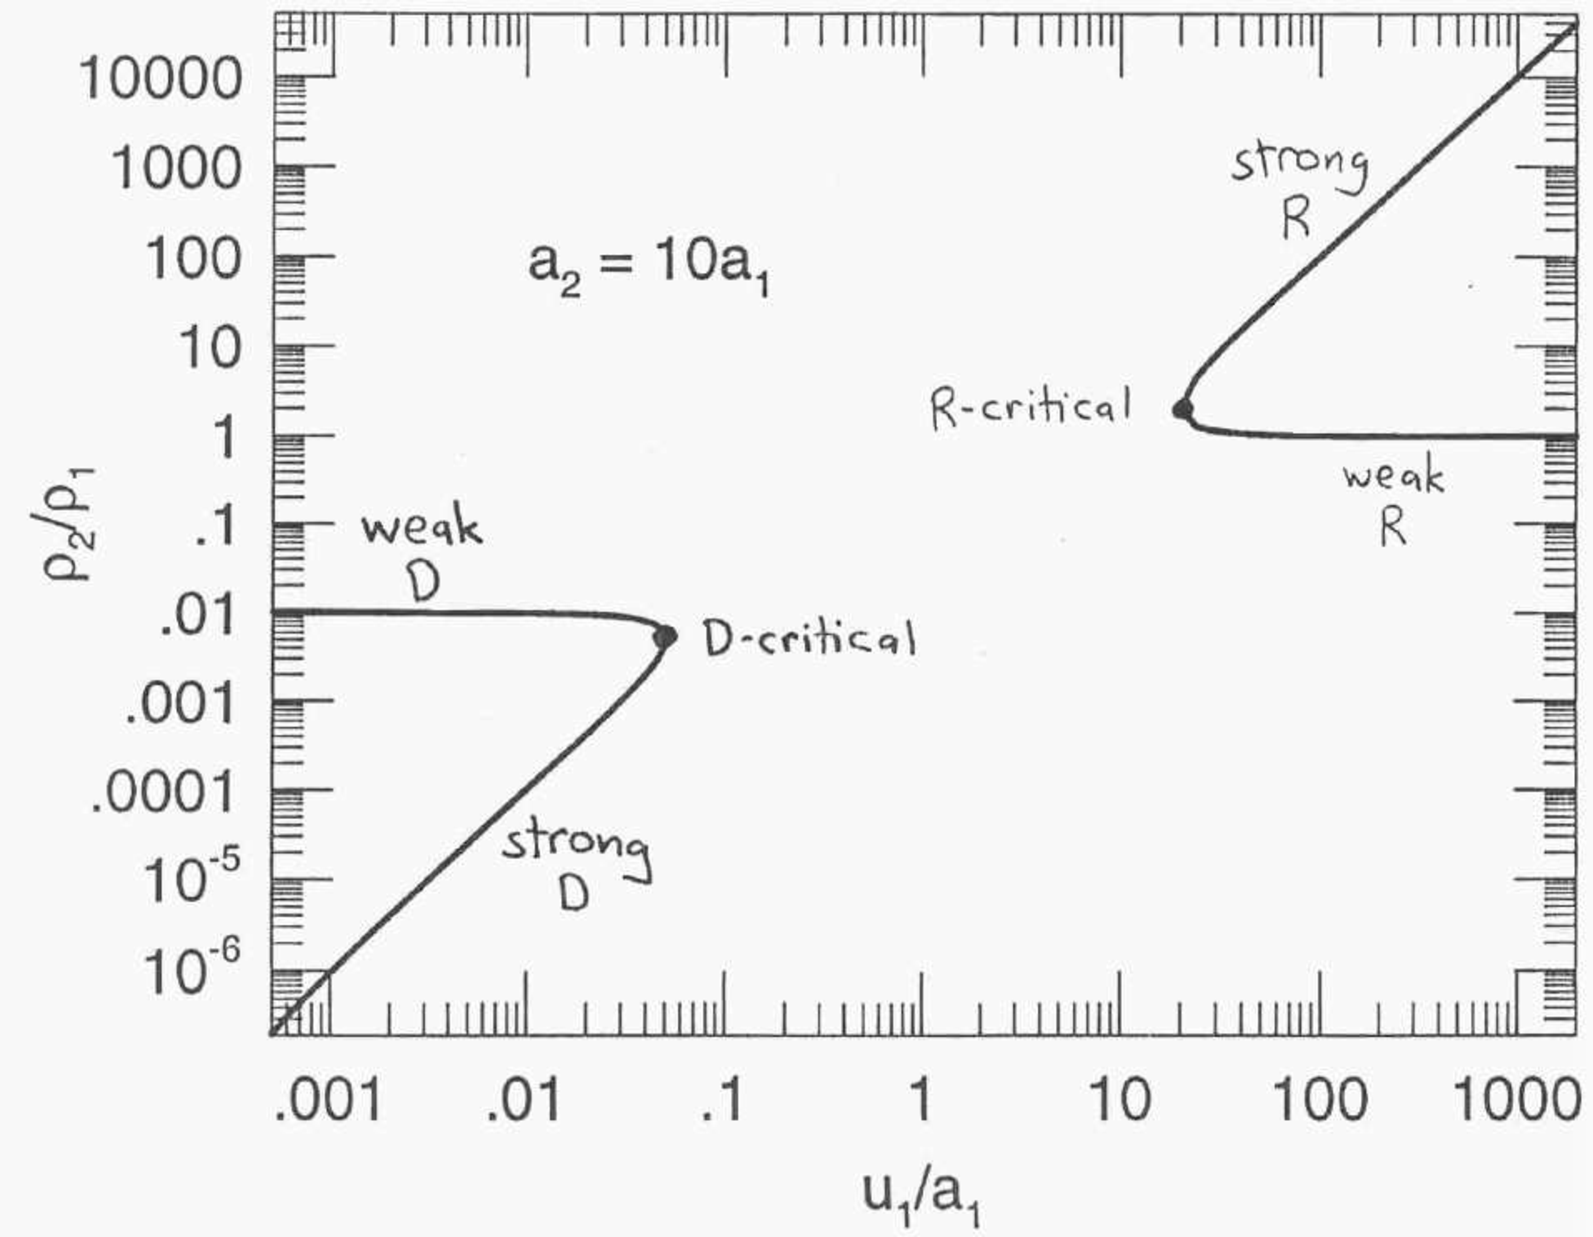
\includegraphics[width=\textwidth]{shock_plot.pdf}
\end{center}
\caption{Density vs. Velocity in an expanding HII region \label{fig:shock}}
\end{figure}

For every ionization front velocity $u_1$, there are two possible density ratios because of the 
plus-minus sign in Eqaution \ref{eq:ratio} (see Figure \ref{fig:shock}.  The larger ratio is a 
\emph{strong front}, and the smaller ratio is a \emph{weak front}.  Strong R-type fronts are 
unstable, but weak R fronts and strong and weak D fronts are observed in HII regions.  In a 
weak front, the ``sonic-ness'' changes (sub to super or super to sub).  In a weak front, 
the sonic-ness does not change.  

Qualitatively, an HII region goes through the following evolution.  When the star first turns on, 
the HII region is small, so the flux of photons is large at the ionization front.  This creates 
a high ionization front velocity $u_1$.  The front in this phase is a weak R-type front.  As 
the ionization front expands, the photon flux decreases, and $u_1$ drops.  When the front slows 
to $u_1=u_R$, the front becomes ``R-critical.''  As $u_1$ continues to drop, an R-type ionization 
front can no longer exist.  At this point, the ionization front becomes D-critical, but the 
shock front remains R-critical and moves ahead of the ionization front (see Figure 
\ref{fig:front}).  The leading shock compresses the neutral gas, and the ionization front then 
ionizes it.  This continues until pressure equilibrium and ionization equilibrium are both 
reached.  At this point
\begin{equation}
R_{final}=\left(\frac{3N_u}{4\pi \alpha n_{final}^2}\right)^{1/3}
\end{equation}
The final density is given by pressure balance:
\begin{equation}
2n_{final}T_2=n_0T_1
\end{equation}
Using the original definition of the Stromgren radius, 
\begin{equation}
R_{final}=\left(\frac{2T_2}{T_2}\right)^{2/3}R_S\sim27R_S
\end{equation}
Before the HII region gets to this point though, the central star will have supernova-ed.  

\begin{figure}[!h]
\begin{center}
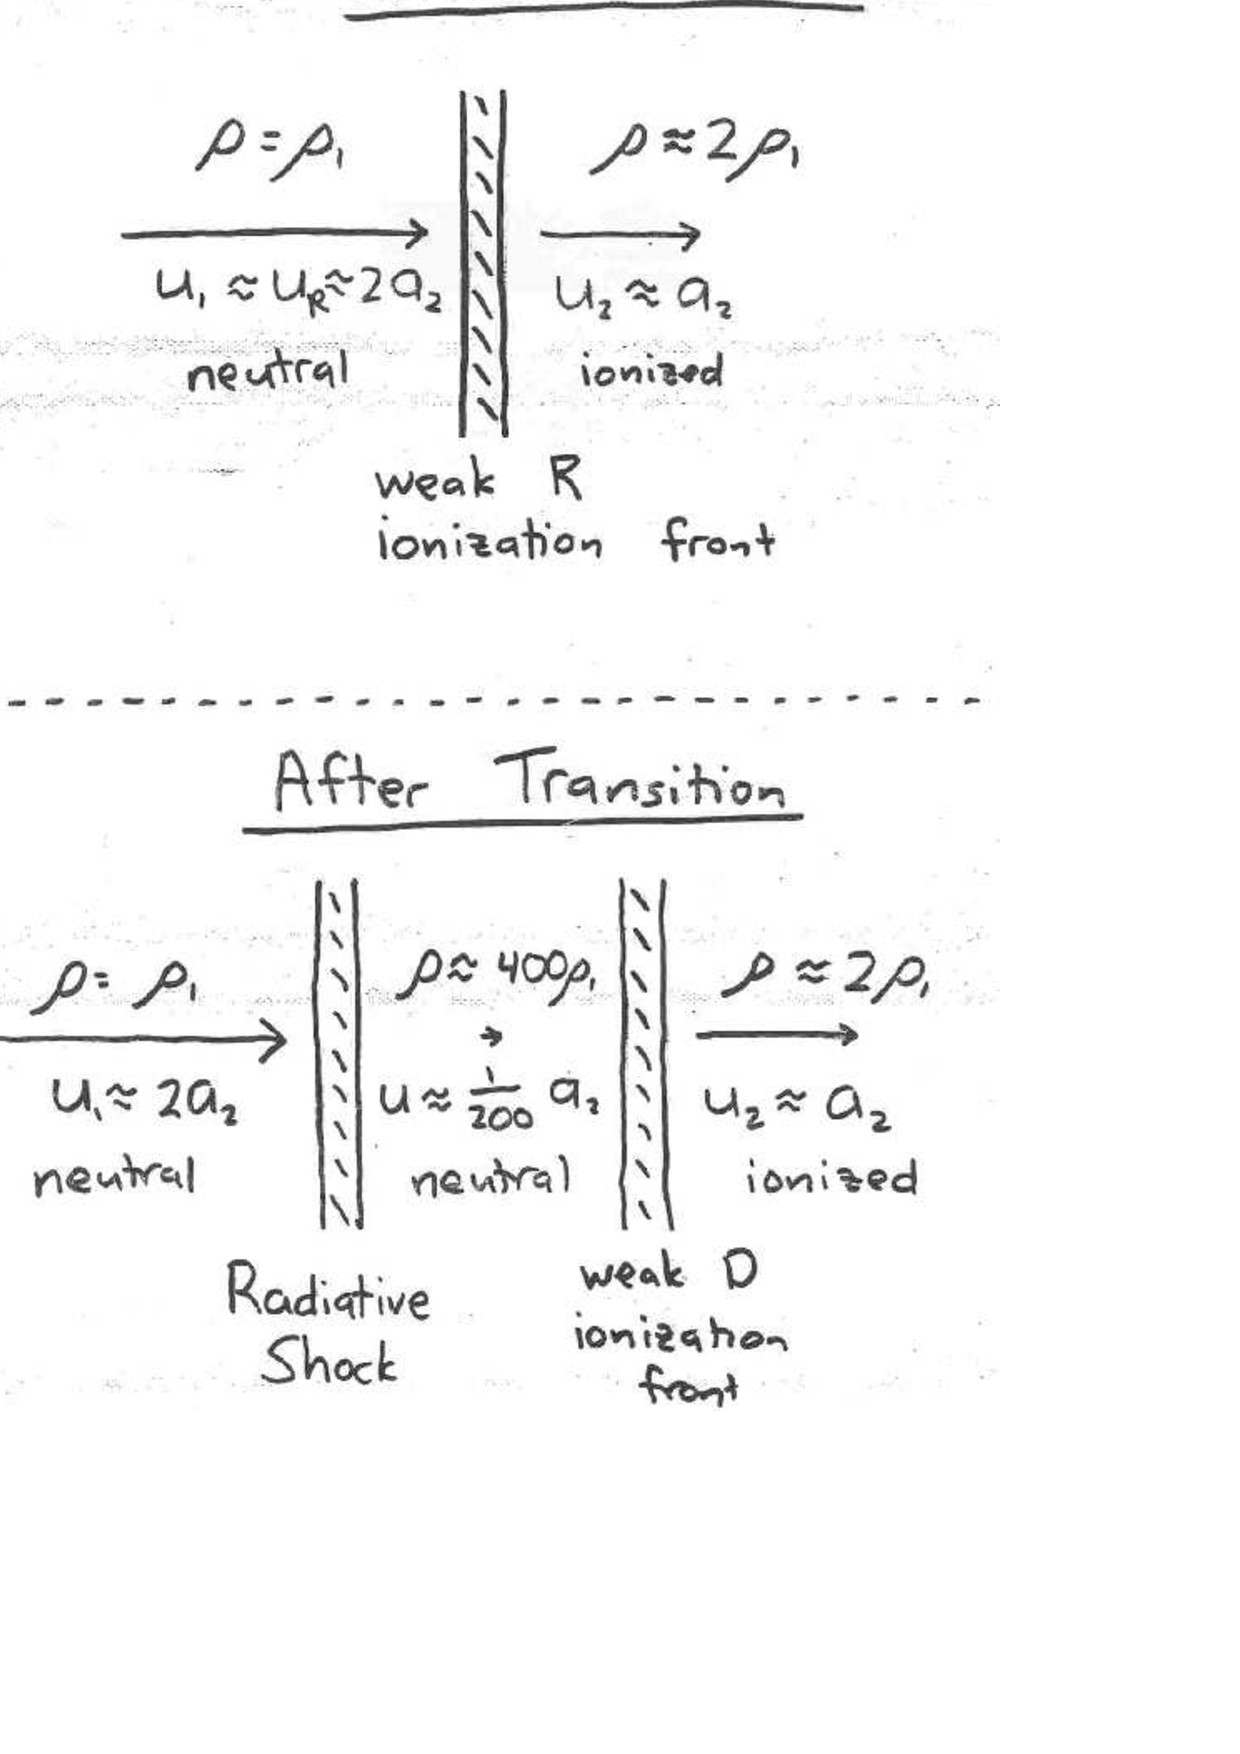
\includegraphics[width=\textwidth]{shock_diagram.pdf}
\end{center}
\caption{Evolution of the shock created by an expanding HII region \label{fig:front}}
\end{figure}

The other thing of interest for HII regions is ionization fraction.  Balancing ionization with 
recombination gives
\begin{equation}
n_{photon}n(1-x)\sigma_{i}c=\alpha x^2n^2
\end{equation}
where x is the fraction of ionized H and n is the total number density of the gas.  The number 
of photons per second coming from the star pass through a volume $4\pi R^2c$, so 
\begin{equation}
n_{photon}=\frac{Q_*}{4\pi r^2c}
\end{equation}
Solving for x and plugging in typical HII region values gives over 99\% ionization (Nutshell 
has an example where $x=0.999983$).  

Also, it might be good to know that the outer parts of an HII region are hotter than the inner 
parts.  This is because the photons that make it to the outer region have a harder spectrum, so 
they can heat the gas more efficiently.  The cross section for H ionization decreases as 
$\nu^{-3}$, so lower energy photons do most of the ionization inside the region.  By the time 
photons reach the outer parts, the lower energy photons have been used up.  

\subsection{Dust}
Dust is formed in the outer layers of AGB stars.  Simple molecules involving 
C or O (depending on the composition of the star) form first.  When the outer 
layers of the star cool to around $1000$ K, gas phase molecules condense onto 
these SiC and SiO seeds, forming more complicated dust molecules.  Based on 
spectra, it is estimated an AGB star ejects $\sim10^8\ M_{\odot}$ of dust 
per year, meaning in the entire galaxy, $\sim10^{-2}\ M_{\odot}$ of dust 
are put into the ISM by AGB stars every year.  

Dust can be destroyed or altered by UV radiation or cosmic rays, as well 
as things like shocks, nearby stars turning on, or anything else that can heat 
interstellar clouds.  For example (we don't actually need to know this, but 
it's hilarious, so I'm including it), lab experiments show that simple ices 
exposed to UV radiation and warmed form an organic ``yellow stuff'' (that's the 
scientific term, check Kwok, it's even in the index!).  When the yellow stuff 
is taken into space and exposed to solar radiation, it turns brown (might I 
suggest another scientific term- ``gets a tan'')

Some facts about dust:

Thermal emission from dust grains is usually in the range of sub-mm wavelengths 
to about $2~\mu m$. Interstellar grains, with temperatures of $10-100$ K, emit
at $30-300\ \mu$m.  Grains near stars have temperatures of a few hundred 
Kelvin, and emit at around $10\ \mu$m.  Dust extinguishes (through both absorption and scattering) background sources in the $0.1-20~\mu m$ range, from UV to mid-IR. This range implies that the sizes of particles is about $0.1-0.2~\mu m$ (see explanation below). Dust also polarizes light, and this has to do with how magnetic fields cause dust grains to align, but someone should help fill in the details here.

Some observational evidence of dust includes the following. One is that low observed abundances of heavy elements, i.e. lower than solar, means that individual metal atoms have been depleted in order to form dust grains. Another is the presence of molecular hydrogen, whose formation if catalyzed on the surfaces of dust grains. Dust also can shield H$_2$ from UV radiation, which prevents it from dissociating as much (Anneila also lists IR absorption lines and diffuse radiation in the galaxy. See notes 5).

Another observational indicator of dust is through the extinction (absorption + scattering) and reddening of the light from background stars.  Scattering by dust roughly follows a $\lambda^{-1}$ law; therefore, shorter bluer wavelengths are more effectively scattered, and light that is transmitted through the cloud appears redder.  An observer not along the dust cloud-star-line-of-sight will receive the shorter bluer wavelengths which were scattered by the dust cloud, and will therefore see a blue reflection nebula.

Extinction from dust, represented by $A_\lambda$, increases the apparent magnitude of an object:

\begin{equation}
m_\lambda = M + 5 \log d - 5 + A_\lambda \,\, .
\end{equation}

Assuming the fractional change in the intensity of light is

\begin{equation}
I_{\lambda} / I_{\lambda,o} = e^{-\tau_{\lambda}},
\end{equation}

\noindent we can combine this with

\begin{equation}
m_1 - m_2 = -2.5 \log_{10} \left(\frac{F_1}{F_2}\right)
\end{equation}

\noindent to show that

\begin{equation}
A_\lambda = 1.086 \tau_\lambda.
\end{equation}

That is, the change in magnitude due to extinction by dust is approximately equal to the optical depth along the line of sight.

\textbf{Mie theory and why dust extinction follows a $1/\lambda$ law}: We can define the extinction coefficient $Q_{\lambda}$ as

\begin{equation}
Q_\lambda \equiv \frac{\sigma_{\lambda}}{\sigma_g}
\end{equation}

\noindent where $\sigma_\lambda$ is the scattering cross section and $\sigma_g = \pi a^2$ is the geometrical cross section of the dust grain.  Mie theory states that in the regime where the wavelength of light $\lambda$ is on the order of the size of the dust grains $a$, then $Q_\lambda \sim a/\lambda$.\sidenote{The derivation of this involves using the complex index of refraction and solving Maxwell's equations with appropriate boundary conditions.  I don't include this derivation here; it can be found in Anneila's notes - Lecture 6, pg. 19.}  Then,

\begin{equation}
\sigma_\lambda \propto \frac{a^3}{\lambda} \quad (\lambda \gtrsim a)
\end{equation}

This is why dust scattering goes as $1/\lambda$, and why dust particles that are about $0.1-0.2$ $\mu m$ effectively extinct background sources in the $0.1 - 20$ $\mu m$ range (UV to mid-IR).  For wavelengths much longer than this, $Q_{\lambda}$ goes to zero.\sidenote{The waves on the surface of water analogy is good for remembering this.  If the wavelength of the waves is much larger than the object through which they are passing, like a grain of sand, then the waves will pass through unobstructed.}  For wavelengths much smaller than this, $Q_\lambda$ becomes independent of $\lambda$, and

\begin{equation}
\sigma_\lambda \propto a^2 \quad (\lambda \ll a).
\end{equation}

Figure \ref{dustextinct} shows some interstellar extinction curves.  These are usually plotted as the ratio of the extinction at a specific wavelength $\lambda$ to the extinction in a reference wavelength ($A_\lambda / A_V$) on the y-axis, and $1/\lambda$ on the x-axis.  At longer wavelengths (left side of the plot), the curve shows a linear increase because the extinction is going as $1/\lambda$ (as we expect from Mie theory).  The bump in the ultraviolet (middle of the plot) is caused by graphite and polycyclic aromatic hydrocarbons.  These are small molecules ($< 0.1$ $\mu m$) that interact strongly with light at 217.5 nm.  Beyond the UV (right side of the plot), the steep increase in the slope of the plot is consistent with Rayleigh scattering\sidenote{Like what happens in the Earth's atmosphere!} $A_\lambda \propto \lambda^{-4}$, where the size of the particles doing the Rayleigh scattering is small, $\leq 0.015$ $\mu m$.

\begin{figure}[h!]
\begin{center}
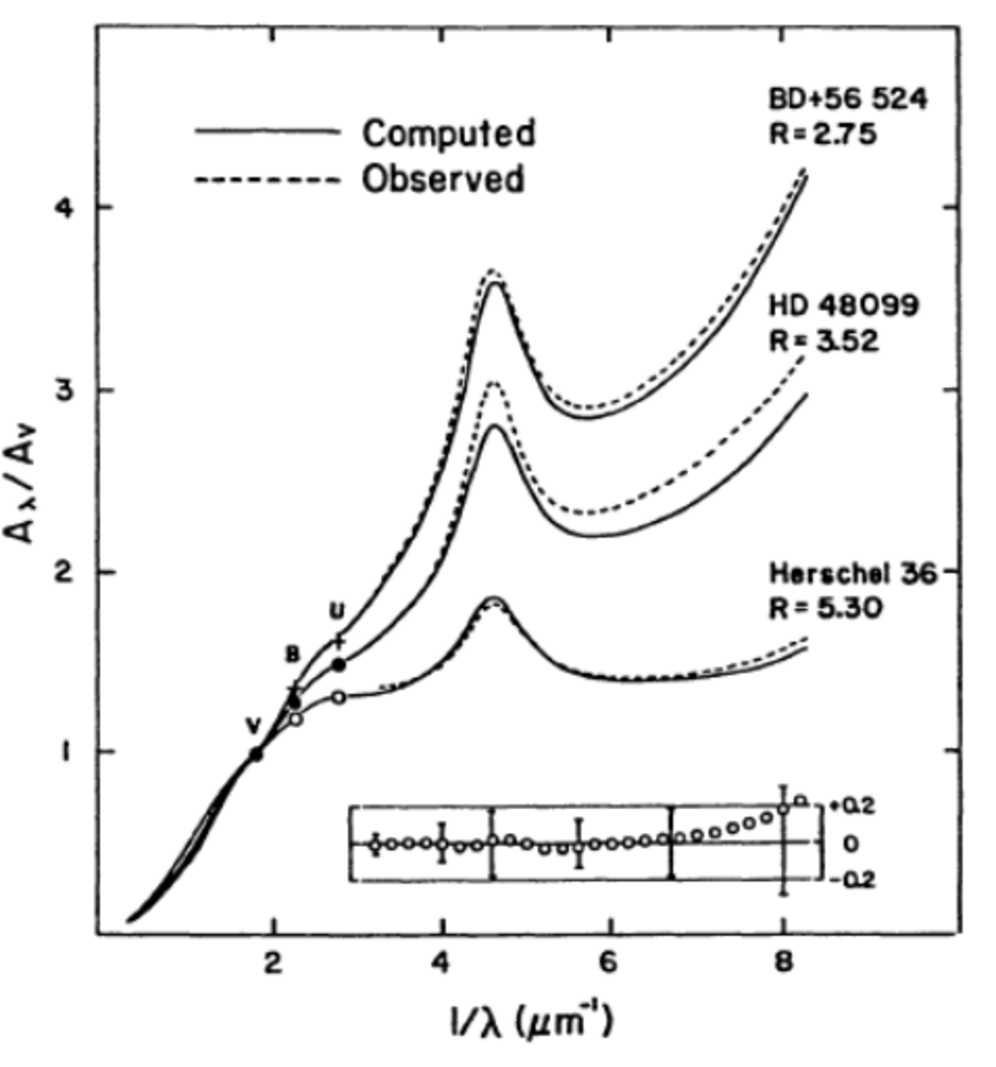
\includegraphics[width=.5\textwidth]{dust_extinction_curve.pdf}\label{dustextinct}
\end{center}
\caption{Interstellar extinction curves.}
\end{figure}

\subsection{Phases of a Supernova}
\newthought{Anneila mentioned that} this was a fairly popular question on the quals, so
I believe a brief review of the phases of a supernova is relevant.  This focuses on the
supernova remnant as opposed to the supernova mechanism itself.  Please edit this if I wrote
something that is wrong or could be explained better -- this is the point of using git.
\begin{enumerate}
    \item The free-expansion phase

    This phase is defined by the fact that the velocity of the ejecta is constant with time. This is also known as ``homologous expansion" because the shape of the density profile remains the same. For every shell of the expanding ejecta, the distance from the source $r = vt$. The condition for being in this phase is that $M_{\rm ejecta} \gg M_{\rm swept}$, that is, the mass swept up by the ejecta from the ISM is not a significant fraction of the ejecta mass.
    The expanding mass of ejecta creates a shock that travels outwards through the ISM
    and a reverse shock that travels inwards through the ejecta.  The reverse shock has a finite
    amount of material to travel through and dies away.
    The outward traveling shock heats the ISM behind it to very high temperatures.
    Thermal bremsstrahlung is seen
    in X-rays, and synchrotron emission is seen in radio from ejected
    particles spiralling around $\mu$G magnetic fields.  This phase ends after 10s to 100s of
    years when the mass of the swept up from the ISM is comparable to the mass of the ejecta.
    Recall that high-mass stars (the progenitors of core-collapse supernovae) typically
    drive large stellar winds.

    \item The adiabatic phase (also called Sedov-Taylor or Blast Wave phase)

    In this phase, the mass of the swept up ISM dominates the mass of the ejected material ($M_{\rm swept} > M_{\rm ejecta}$).
    However, the density of the material behind the shock is not yet large enough for cooling
    to be significant.  Therefore, the gas expands adiabatically.
    From dimensional analysis considerations, we can derive the Sedov-Taylor solution which says
    \begin{dmath}
        R \sim \left(\frac{Et^2}{\rho}\right)^{1/5}
    \end{dmath},
    where $R$ is the radius of the supernova remnant, $E$ is the energy released by the
    supernova, and $\rho$ is the density of the surrounding ISM. The Sedov phase usually lasts about $10^4$ years.

    \item The radiative phase (or snowplow phase)
    
    This is also called the momentum-conserving phase. Consider a shell with mass $M_s$ and velocity $v_s$. The momentum $p_0 = M_s v_s$ is constant, giving the equation of motion
    \begin{equation}
    p_0 - \biggl(\frac{4}{3}\pi R^3 \rho_0 \biggr) \dot{R}\,\, ,
    \end{equation}
    which can be integrated to show that
    \begin{equation}
    R \propto t^{1/4}\,\,.
    \end{equation}
    \item Merger with the ISM
    
    Occurs when $v_s = c_s$ is the sound speed.
\end{enumerate}

\subsection{The Fluid Equations}
The following are the ideal or ``inviscid" fluid equations.

Mass conservation:
\begin{equation}
\frac{\partial \rho}{\partial t} + \vec{\nabla} \cdot \rho \vec{v} = 0
\end{equation}

Momentum conservation:
\begin{equation}
\frac{\partial}{\partial t} (\rho \vec{v}) + \vec{\nabla}\cdot (\rho \vec{v} \vec{v}) = -\vec{\nabla} P + \rho \vec{f}
\end{equation}

Energy conservation:
\begin{equation}
\frac{\partial}{\partial t} \biggl( \frac{1}{2} \rho v^2 + \rho \epsilon \biggr) + \vec{\nabla}\biggl[\biggl(\frac{1}{2}\rho v^2 + \rho \epsilon \biggr) + P \vec{v} \biggr] = \rho \vec{f} \cdot \vec{v}\,\,.
\end{equation}
The right-hand side of this equation is the work done by external forces (other people should feel free to add to this section or add different forms of the equations). Also, the Lagrangian or ``comoving" time derivative is

\begin{equation}
\frac{d}{dt} = \frac{\partial}{\partial t} + (\vec{v} \cdot \vec{\nabla})\,\, ,
\end{equation}
where $\frac{\partial}{\partial t}$ is the Eulerian time derivative, not comoving with the fluid.

It's probably good to know basically how to do perturbation theory on these equations, which you can do by saying $\rho \rightarrow \rho_0 + \delta \rho$ and the same with $P$ and $v$ (assume $v_0 = 0$), then killing all the terms that are second-order in $\delta$ quantities.

It's also a good idea to know Bernoulli's equation:
\begin{equation}
(\vec{v}\cdot \vec{\nabla})\biggl(\frac{1}{2} v^2 + h + \phi \biggr) = 0\,\, .
\end{equation}
or
\begin{equation}
\frac{1}{2} v^2 + h + \phi = {\rm constant}
\end{equation}
along every streamline. The first term is kinetic energy, the second is gravitational potential energy, and and third is thermal energy $+$ work that can be done.

\subsection{Shocks}
Adiabatic shocks:\newline
Shocks form easily in astrophysical enviroments because gravity can accelarate 
gas to large velocities, but the cold gas in the ISM has a low sound speed.  
The ratio of flow velocity to sound speed is called the Mach number:
\begin{equation}
\boxed{M=\frac{v}{c_s}}
\end{equation}
A shock forms when the bulk flow of a fluid is faster than the sound speed in the 
gas, and the gas is decelerated by another fluid.  Since the fluid is 
moving supersonically, the next layer of the fluid hits the decelaration before 
information about the decelaration can reach it from the previous layer.  So 
the fluid cannot adjust slowly to the decelaration, and a discontinuity forms.  
This is a shock.  

Adiabatic Shocks:\newline
The jump conditions across a shock can be derived using the 1-D fluid 
continiuity equations across the shock boundary.  In the frame of the shock, 
fluid is coming at the shock from region 1 and leaving the shock into region 2.  
Consider a thin layer d$x$ around the shock.  Starting with mass continuity:
\begin{equation}
\frac{\partial \rho}{\partial t}+\frac{\partial}{\partial x}(\rho u_x)=0
\end{equation}
Mass is not accumalted in the layer d$x$, so 
$\frac{\partial \rho}{\partial t}=0$.  This implies 
$\frac{\partial}{\partial x}(\rho u_x)=0$, so 
\begin{equation}
\boxed{\rho_1u_2=\rho_2u_2}
\end{equation}
Similarly, the momentum energy conservation equations (assuming an adiabatic 
shock) give 
\begin{equation}
\boxed{\rho_1u_1^2+p_1=\rho_2u_2^2+p_2}
\end{equation}
\begin{equation}
\boxed{\frac{1}{2}u_1^2+\epsilon_1+\frac{p_1}{\rho_1}=\frac{1}{2}u_2^2+\epsilon_2+\frac{p_2}{\rho_2}}
\end{equation}
These are the Rankine-Hugoniot jump conditions.  The energy condition can 
be put into a more convenient form by substituting for $\epsilon$, the internal 
energy per unit mass.  The fluid is brought to $\epsilon$ by $p$d$V$ work (it's 
adiabatic), so
\begin{equation}
\epsilon=\frac{pdV}{m}=K\rho^{\gamma}d(1/\rho)=\frac{1}{\gamma-1}\frac{p}{\rho}
\end{equation}
Then
\begin{equation}
\frac{1}{2}u_1^2+\frac{\gamma}{\gamma-1}\frac{p_1}{\rho_1}=\frac{1}{2}u_2^2+\frac{\gamma}{\gamma-1}\frac{p_2}{\rho_2}
\end{equation}
Assuming $\gamma$ does not change across the shock.  Using 
$=\gamma\frac{p}{\rho}$,
\begin{equation}
\frac{1}{2}u_1^2+\frac{c_1^2}{\gamma-1}=\frac{1}{2}u_2^2+\frac{c_2^2}{\gamma-1}
\end{equation}
Now follows a bunch of messy algebra that we probably don't need to know, but 
look at pages 82 and 83 of Clark and Carswell if you're interested.  
The result is that 
\begin{equation}
\frac{\rho_2}{\rho_1}=\frac{(\gamma+1)p_2+(\gamma-1)p_1}{(\gamma+1)p_1+(\gamma-1)p_2}
\end{equation}
In a strong shock, $p_1$ is negligible, and this expression becomes
\begin{equation}\label{eq:den}
\boxed{\frac{\rho_2}{\rho_1}=\frac{\gamma+1}{\gamma-1}=4}
\end{equation}
assuming $\gamma=5/3$.  The compression of the fluid is limited because of 
the adiabatic assumption.  As the shock gets stronger, the thermal pressure 
of the post-shocked gas increases, which prevents additional compression.  
If the thermal energy could be released, this wouldn't happen, but we assumed 
the shock is adiabatic.  

Using the second jump condition, and neglecting $p_1$, 
\begin{equation}
P_2=\rho_1u_1^2-\rho_2u_2^2=\rho_1u_1^2-\rho_1u_1^2/4=\frac{3}{4}\rho_1u_1^2
\end{equation}
This can be used with Equation \ref{eq:den} and the ideal gas law to show 
\begin{equation}
\boxed{T_2=\frac{3\mu m_H u_1^2}{16k}}
\end{equation}
For typical shock velocities of $100$ km/s, this corresponds to post-shock 
temperatures of $\sim10^5$ K.  Also of interest is the Mach number of the 
post-shocked gas.  
\begin{equation}
M_2^2=\frac{u_2^2}{c_2^2}=
\frac{\rho_2}{\gamma p_2}\frac{u_1^2}{16}=
\frac{u_1^2}{16}\frac{4\rho_2}{3\gamma\rho_1u_1^2}=
\frac{1}{3\gamma}=
\frac{1}{5}
\end{equation}
So the post-shocked gas moves subsonically.

Isothermal Shocks:\newline
The other limiting case of shocks is an isothermal shock.  In an isothermal 
shock, the shocked gas cools to its pre-shock temperature.  This 
happens over a cooling length that is much less than the lengthscale of the 
system.  The immediate post-shock will be adiabatic, but if this is over a 
small enough length, the adiabatic portion can be lumped is as part of the 
shock and ignored.  The continuity conditions can then be applied to the 
pre-shock and isothermal part of the post-shock.  The first two jump conditions 
still hold, but the energy conserving one no longer applies.  Instead, it is 
replaced by 
\begin{equation}
\boxed{T_1=T_2}
\end{equation}
Since the shock is isothermal, the sounds speed before and after is the same.
\begin{equation}
c_s^2=\frac{p}{\rho}
\end{equation}
The momentum jump condition then gives
\begin{equation}
\rho_1(u_1^2+c_s^2)=\rho_2(u_2^2+c_s^2)
\end{equation}
Substituting the mass jump condition for $\rho_1$ and rearrangeing gives
\begin{equation}
(u_2-u_1)c_s^2=u_1u_2(u_2-u_1)
\end{equation}
Therefore
\begin{equation}
c_s^2=u_1u_2
\end{equation}
and 
\begin{equation}
\boxed{\frac{\rho_2}{\rho_1}=\frac{u_1}{u_2}=\left(\frac{u_1}{c_s}\right)^2=M^2}
\end{equation}
So there is no limit to how much a strong shock can compress the gas.  
Note that because $c_s^2=u_1u_2$ and $u_1>c_s$ by definition of a shock, the 
post-shocked gas is subsonic.  

Magnetic Fields in Shocks:\newline
This is based on the class notes, so I'm going to be making some statements 
that seem to come out of thin air (just like they do in the notes).  Someone 
who has a better reference or understands this better should fill in the 
details.  

In the presence of magnetic field, magnetic pressure must be included in 
the momentum conservation equation across a shock of a plasma.  
\begin{equation}
P_1+\rho_1v_s^2+\frac{B_1^2}{8\pi}=P_2+\rho_2u_2^2+\frac{B_2^2}{8\pi}
\end{equation}
Assuming that in the pre-shock gas, ram pressure dominates and in the post-
shock gas, magnetic pressure dominates, this becomes
\begin{equation}\label{eq:B2}
B_2^2=8\pi\rho_1v_s^2
\end{equation}
Because the magnetic field lines are frozen into the plasma and magnetic flux 
$B/\rho$ is through a ``circuit'' of the plasma is conserved, the presence 
of the magnetic field reduces the compression of the gas by the shock.  
By flux conservation:
\begin{equation}
B_2=B_1\frac{\rho_2}{\rho_1}
\end{equation}
Combining this with Equation \ref{eq:B2} and solving for the density ratio gives
\begin{equation}
\left(\frac{\rho_2}{\rho_1}\right)^2=2\times\frac{4\pi\rho_1v_s^2}{B_1^2}=2\frac{v_s^2}{v_a^2}
\end{equation}
where $v_a$ is the \emph{Alfven velocity}, defined as
\begin{equation}
v_a\equiv\frac{B}{(4\pi\rho)^{1/2}}
\end{equation}
The Alfven Mach number is then defined as 
\begin{equation}
M_A\equiv\frac{v_s}{v_A}
\end{equation}
With this definition, 
\begin{equation}
\frac{\rho_2}{\rho_1}=\sqrt{2}M_A
\end{equation}
In the presence of a magnetic field, disturnbance propogate at the Alfven 
velocity, not at the sound speed.  

In a gas containing a mix of ions and neutrals, a magnetic field will affect 
the structure of a shock.  Only the ions feel the magnetic field, but they 
can transfer the effects to the neutrals through collisions.  The shock 
structure depends on the strength off the magnetic field.  A magnetic 
precursor to the shock with smooth out the velocity disontinuity for the ions 
(see Figure \ref{fig:Cshock}).  The magnetic field does not want to 
suddenly change strength (and therefore flux), so it pushes the ions away from 
the shock, smoothing their velocity and density change into the shock.  
In a very weak magnetic field, the ions will 
have a small warning off the shock, and will feel less of a discontinuity, 
while the neutrals will be uneffected and feel a normal \emph{J-shock}.  For 
increasingly strong magnetic fields, the ions will have more warning and 
their discontinuity will be increasingly smoothed out.  With the additional 
warning time, the ions will have more time to collisionally change the 
neutral velocity, smoothing out the neutral discontinuity as well.  If the 
magnetic field is strong enough, the J-shock of the neutral will turn into 
a completely smooth transition known as a \emph{C-shock}.

\begin{figure}[!h]
\begin{center}
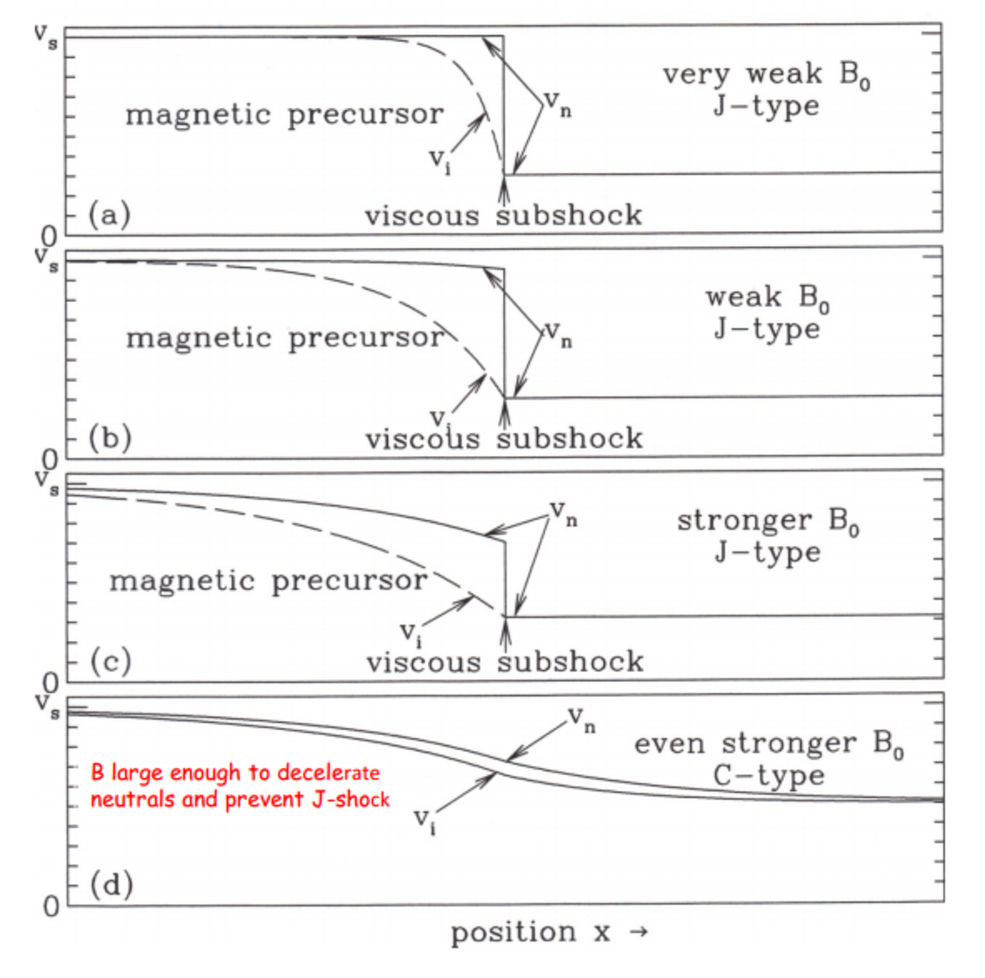
\includegraphics[width=\textwidth]{Cshock.pdf}
\end{center}
\caption{Shocks involving magnetic fields. \label{fig:Cshock}}
\end{figure}

\subsection{Magnetic Fields}
Applications of magnetic fields is covered in shocks and in star formation.  

Observational evidence of interstellar magnetic fields include polarization 
of starlight, the Zeeman effect, and pulsar faraday rotation measurements.  
Polarization of starlight is caused by non-sherical dust grains.  These dust 
grains can be modeled as cylinders rotating end over end, with their short 
axis parallel to the B field.  Observations indicate ISM B fields of order 
$10^{-6}$ gauss.  The Zeeman effect can be observed as hyperfine splitting 
of the $21$ cm H line due to the B field.  The frequency difference between 
the two lines is $\frac{eB}{4\pi m_ec}\sim3\times10^6B Hz$, so this is 
difficult to observe for B fields of $10^{-6}$ gauss.  

Faraday rotation is the rotation of linearly polarized light to a different 
linear polarization as it passes through a plasma with a magnetic field going 
through it (see section in radiative processes).  The amount of rotation, which 
can be measured as a function of frequency, is 
$\propto \int_0^L n_eB$, so a measure of rotation gives the product of density 
and magnetic field.  The density can be determined using dispersion, a measure 
of the time delay in a signal as a function of frequency.  This is proportional 
to $\int_0^L n_e$.  So by measuring Faraday rotation and dispersion, B can 
be determined.  Pulsar observations using this technique find a B field 
strength also of order $10^{-6}$ gauss. 

\subsection{Star Formation}
I think most of what we need to know about star formation is in the Stars 
section of the notes.  The only thing new here is magnetic fields.  

Most molecular cloud cores are Jeans-unstable to collapse, but star formation 
efficiency is lower than it should be if this is true.  The angular momentum 
and magnetic flux in stars is lower than that in clouds, so angular momentum 
and magnetic flux must be lost during collapse.  Also, collapsing clouds are 
not as flat as theory predicts, and have broadened lines implying some sort 
of turbulence.  All this implies magnetic fields play an important role in star 
formation.  \emph{Ambipolar diffusion} delays cloud collapse and provides a way 
for magnetic flux to be lost.  The Alfven waves produced in this process 
cause turbulence, which can broaden spectral lines (the notes just state these 
things without justifying them).   

Even in a cold molecular cloud core, this is a small fraction of ionization.  
The ionized particles are frozen to the magnetic field lines, which prevents 
them from collapsing.  The neutral particles don't care about the magnetic 
field lines, but they do have diffuse through the trapped ions in order to 
collapse.  The force per unit volume $f$ on the neutrals from collions with the 
ions is the collision rate per unit volume times the change in momentum 
of a neutral per collision.  So $f$ is given by
\begin{equation}
f=n_in_n<v\sigma>m_n(u_i-u_n)
\end{equation}
Here, $u_i-u_n$ is the velocity of the neutrals relative to the ions and field 
lines.  Therefore, this is also the velocity with which the neutrals drift 
across the magnetic field lines, $v_D$.  Balancing the collisional force with 
gravity:
\begin{equation}
\rho\frac{GM}{r^2}=n_in_n<v\sigma>m_nv_D
\end{equation}
\begin{equation}
n_nm_n\frac{GM}{r^2}=n_in_n<v\sigma>m_nv_D
\end{equation}
\begin{equation}
\frac{GM}{r^2}=n_i<v\sigma>v_D
\end{equation}
The left hand side can be rewritten as
\begin{equation}
\frac{GM}{r^2}=\frac{GM}{r^3}r=\frac{4\pi}{3}Gn_nm_nr
\end{equation}
So
\begin{equation}
\frac{4\pi}{3}Gn_nm_nr=n_i<v\sigma>v_D
\end{equation}
\begin{equation}
v_D=\frac{4\pi}{3}\frac{Gn_nm_nr}{n_i<v\sigma>}
\end{equation}
The timescale for ambipolar diffusion is 
\begin{equation}
t_D=\frac{r}{v_D}=\frac{3n_i<v\sigma>}{4\pi Gn_nm_n}\sim7\times10^{13}\frac{n_i}{n_n} years
\end{equation}
I'm not sure where the numbers being plugged into this come from.  For 
molecular cloud cores, $n_i/n_n\lesssim10^{-6}-10^{-5}$, so the diffusion time 
is $\lesssim10^7$ years.

\subsection{ISM in Other Galaxies}
The following is taken from slide 21 on February 28.  I don't really understand 
it, but it get's an entire slide to itself, so it must be important...

AGN       ?'s.....

The other galaxies stuff is all from Nick's slides, so most of what he 
shows is example spectra and images.  Not really sure what to do with that, 
but he's on the committee and this is what he does research on, so he might 
ask about it.  If anyone has a better reference for this stuff, feel free 
to add to this section.  The main topics seem to be special types of galaxies 
like AGN and galaxies with lots of star formation.  AGN will be covered in High Energy with better detail, 
so I'll skip that for now.  

Star formation happens in starburst galaxies, where a recent galaxy merger 
forces large amounts of gas into the center, triggering star formation.  
If the star formation is obscured by dust, the dust re-emitts at longer 
wavelengths and you see an ULIRG (Ultra-Luminous Infrared Galaxy) or a sub-mm 
galaxies.  This is about all I know off the top of my head, and I can't figure 
out anything useful from Nick's notes.  I think this topic is partially covered 
in the Galaxies will-ask though, and may also be covered in George's cosmology 
topics.  
